\chapter{Literature Review}


% source of cr & introduce acceleration mechanism
Cosmic-ray could come from different origins from galactic sources
to extra-galactic sources. The kinetic energy of cosmic rays also 
highly depends on where does it from. Low energy CRs usually came from 
the Sun called ``solar energetic particle''. The production process of 
soalr particle event mostly came from the coronal mass ejection (CME)
when HZE ions were dragged by a magnetic field in the plasma.
The extra-galactic CRs typically 
has high momentum from the extreme condition of the acceleration mechanism
in pulsar, quasars and supernova remnant (SNR). 
The theoretical description of acceleration in SNR and solar flares
is the shock wave acceleration in the following paragraph.

% acceleration mechanism
One of the most impactful studies of CR's acceleration mechanism 
was conducted by \cite{fermi1949origin}. 
The study describes how high energy CR particle gain such a huge 
momentum from the shock wave that was generated by supernovae 
or a great explosion from the heavy dense star. How it gains
the kinetic energy could be described as a first-order shock 
acceleration and the overall spectrum of charged particles could be
represented as the power law in Equation \ref{eq:fermi_powerlaw}.

\begin{equation}
    \frac{dN(E)}{dE} \propto E^{-\gamma}
    \label{eq:fermi_powerlaw}
\end{equation}
where $\gamma \geq 2$ in the non-relativistic regime.
However, moving magnetized plasma cloud can accelerate the charged particle in the space called "second-order Fermi acceleration".
Both regimes were computed the Lorentzian forces regardless of thermal collision in the process.

% cosmic ray component paper
The CR protons are major components in the arrival of CR particles under multiple observations. However, $\alpha$-particle is also 
a second important CR particle when considering a precise calculation
of CR interactions. The other majority of heavy weight nuclei that could propagate through space are C, O, Ne and so on. 
The differential flux in kinetic energy of multiple observations is 
visualzed in the Figure \ref{fig:cr_composition} under the work of 
\cite{review_particle_physics2012} to take various atomic nnumbers 
from various experiments.

\begin{figure}[h!]
    \centering
    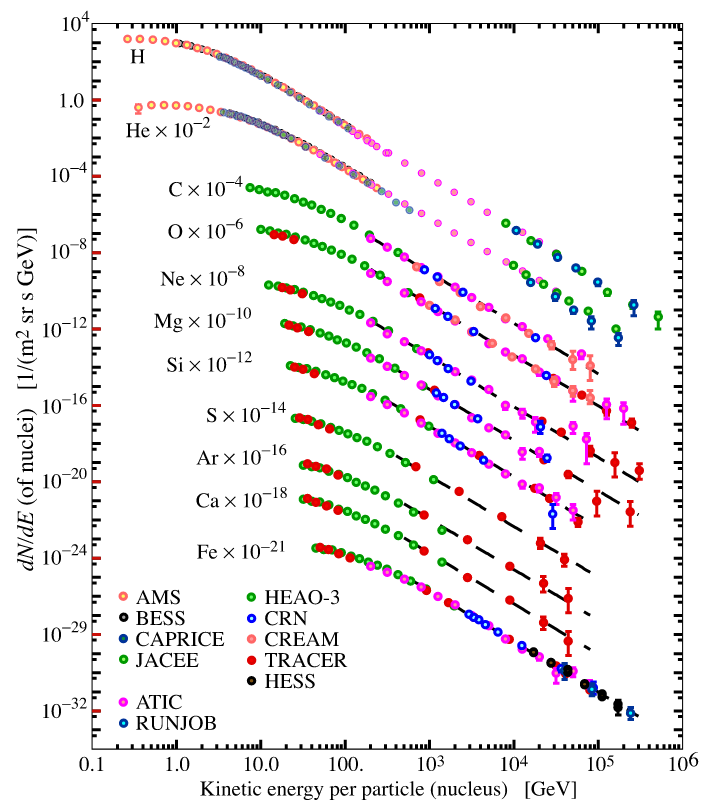
\includegraphics[width=0.6\textwidth]{content/literature_review/figures/cr_composition.png}
    \caption{Cosmic-ray elemental spectra from various experiments (\cite{review_particle_physics2012})}
    \label{fig:cr_composition}
\end{figure}


% CR and Earth's magnetic field -> cutoff rigidity
% ctte -> cutoff rigidity
Since there is a moving plasma inside the Earth, the magnetic field 
has been generated from the dynamics of the moving charged ions in 
the plasma. The magnetic field of the Earth has a north pole at 
the geometric south pole of the Earth and vice versa. 
The Earth's magnetic field play
an important role in the arrival of CR particles because the Lorentzian 
forces will bend the direction of a moving charged particle depends 
on the rigidity of the particle.
This means the magnetic field line mantles the Earth with a
certain direction towards the geometric north pole.

% cite -> east-west
Firstly, it creates the CR cutoff rigidity on the terrestrial
where each location of the Earth requires a minimum rigidity of incident charged particles as a condition for arrival. The 
Figure \ref{fig:cr_map_rigidity} shows a cutoff rigidity on the Earth's surface.

\begin{figure}[h!]
    \centering
    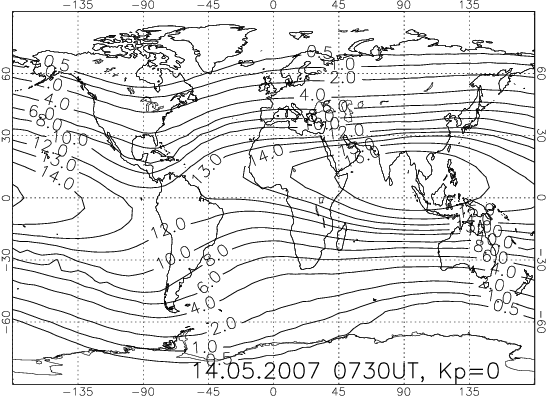
\includegraphics[width=0.6\textwidth]{content/literature_review/figures/map_cutoff_rigidity.png}
    \caption{ World map with computed geomagnetic vertical cutoff
        rigidity contour lines on a given date
        (\cite{map_cr_rigidity_cutoff})
    }
    \label{fig:cr_map_rigidity}
\end{figure}

%  east-west and Explorer XI first observe cite{kraushaar1965explorer}
Secondly, incoming charged CRs with a charge has been dragged 
by the Earth's magnetic. Then a charged particle would move as 
a curve or a spiral depends on the rigidity of an incoming particle
which leads to the East-West effects when an orbiting detector could 
find more particle on the Westside more than on the East side for 
a significant level of intensity. A pioneer Earth's $\gamma$-ray 
experiment is conducted by \cite{kraushaar1965explorer} where the 
detector was deployed on the Explorer XI satellite and orbiting in the sky.


% east west : Kraushaar65 Kraushaar72
\begin{figure}[h!]
    \centering
        \subfloat[
            Explorer XI (\cite{kraushaar1965explorer})
        ]{
            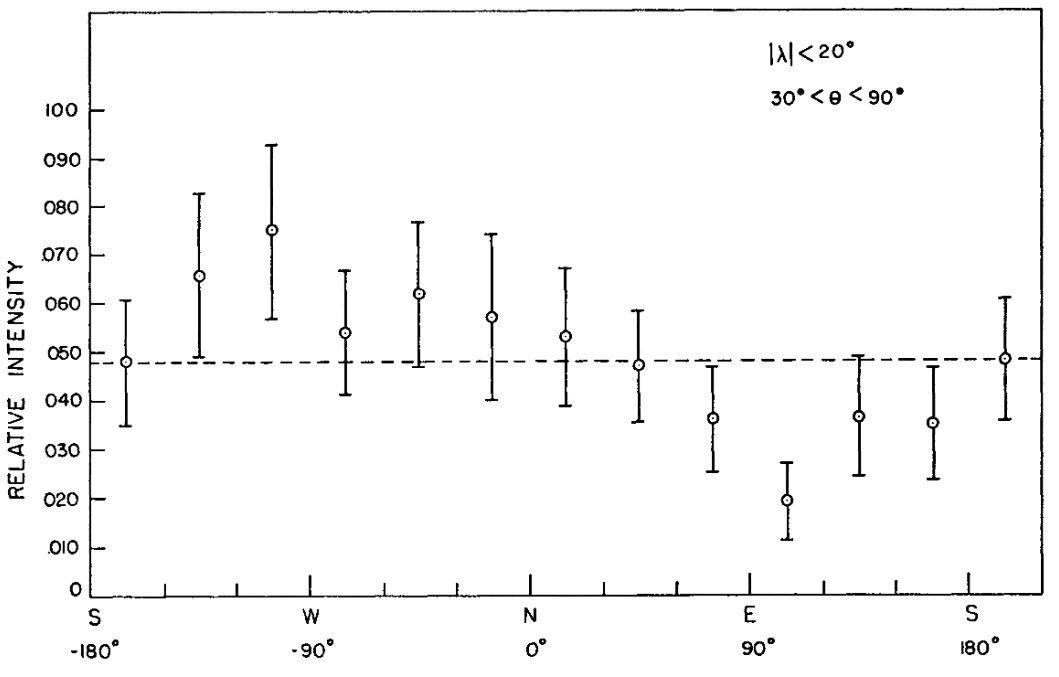
\includegraphics[width=0.48\textwidth]{content/literature_review/figures/explorer_xi_eastwest.png}
            }
        \hfill
         \subfloat[
            OSO-3 (\cite{Kraushaar72})
         ]{
            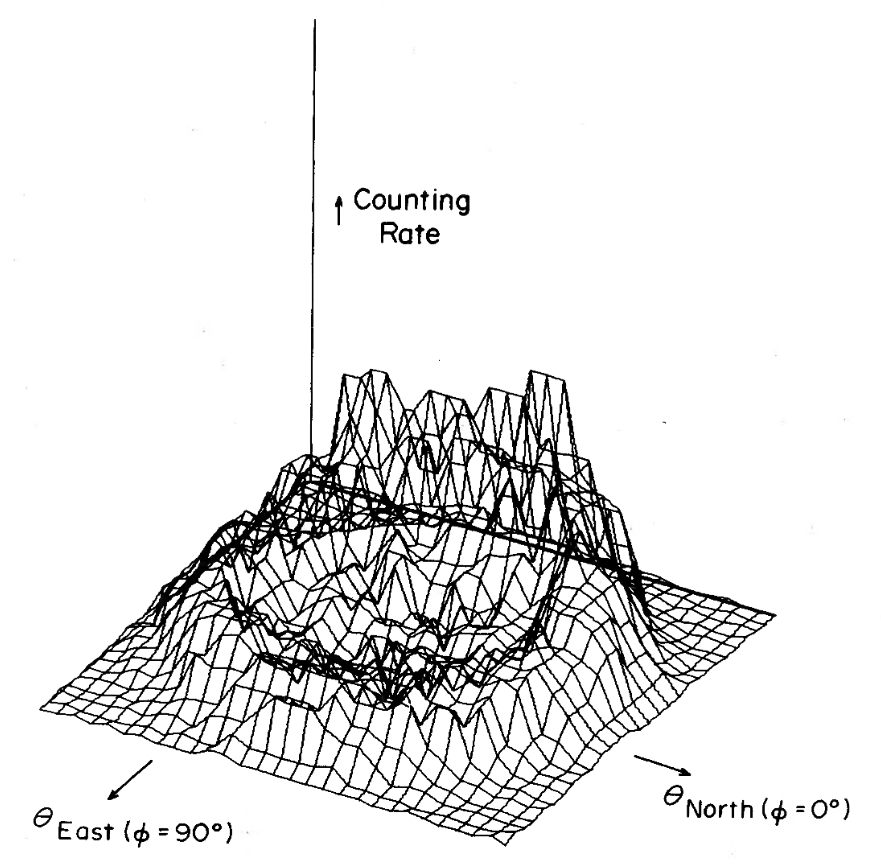
\includegraphics[width=0.48\textwidth]{content/literature_review/figures/eastwest_1972}
        }
        \caption{
            The asymmetry of $\gamma$-rays East-West intensity 
        }
       \label{fig:gamma_ew}
\end{figure}
The incoming photon from the East and West direction is the crucial evidence 
of the bending of CRs trajectory by Earth's magnetosphere. The first 
analysis shows a distinguishable intensity from East to West as visualized 
in Figure \ref{fig:gamma_ew}a. The second experiment where
the $\gamma$-ray detector is attached on Third Orbiting Solar
Observatory (OSO-3) and collecting the $\gamma$-ray in MeV range.
The 2-D plot of the intensity is shown in Figure \ref{fig:gamma_ew}b.

% describe zenith
Moreover, An early analysis found 
that the observing $\gamma$-rays intensity along the zenith angle
from different geomagnetic latitude ($\lambda$) is differentiable
as shown in Figure \ref{fig:explorer_xi_zenith}. The reason behind 
this outcome came from the Earth's rigidity where the incoming 
particles near the equatorial have less chance to arrive than the 
north pole and likely to interact with the atmospheric molecules 
and emits the $\gamma$-rays. This is the secondary 
evidence of how geomagnetic fields play an important role on the 
trajectory of the CR particles. 

\begin{figure}[h!]
    \centering
        \subfloat[
            observing above 20\textdegree geomagnetic latitude 
        ]{
            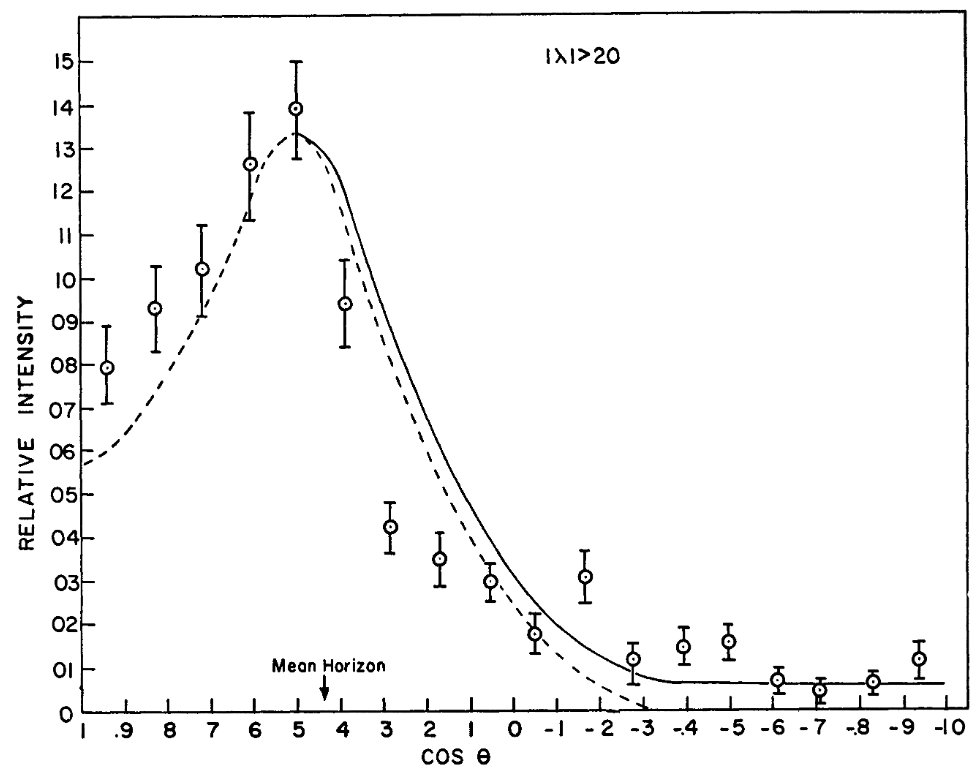
\includegraphics[width=0.48\textwidth]{content/literature_review/figures/explorer_xi_azimutal_lambda_a20.png}
            }
        \hfill
         \subfloat[
            observing below 20\textdegree geomagnetic latitude 
         ]{
            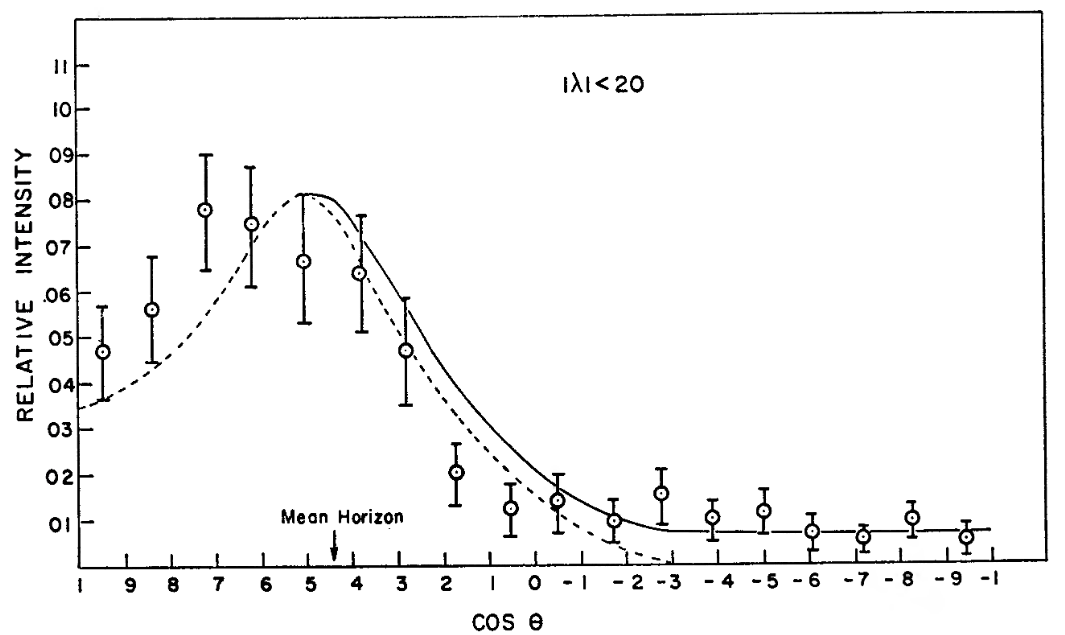
\includegraphics[width=0.48\textwidth]{content/literature_review/figures/explorer_xi_azimutal_lambda_b20.png}
        }
        \caption{
            $\gamma$-ray intensity along the zenith angle
            (\cite{kraushaar1965explorer})  
        }
       \label{fig:explorer_xi_zenith}
\end{figure}

% early earth gamma-ray observe -> SAS-2 (Thompson81),  EGRET (Petry05)
The following experiment of Earth's albedo observations is conducted 
by sending a second small astronomy satellite (SAS-2) with a higher 
resolution in angle and observing above 35 MeV up to GeV range
(\cite{Thompson81}). The projected 3-D representation of intensity
is shown in Figure \ref{fig:gamma_earth_second_wave}a. A few decades 
later, another precise $\gamma-ray$ detector has been attached in the 
CGRO satellite (\cite{Petry05}). An outcome from the analysis illustrated the bright region around the Earth's limb region as 
in Figure \ref{fig:gamma_earth_second_wave}b.


\begin{figure}[h!]
    \centering
        \subfloat[
            SAS-2 experiment (\cite{Thompson81})
        ]{
            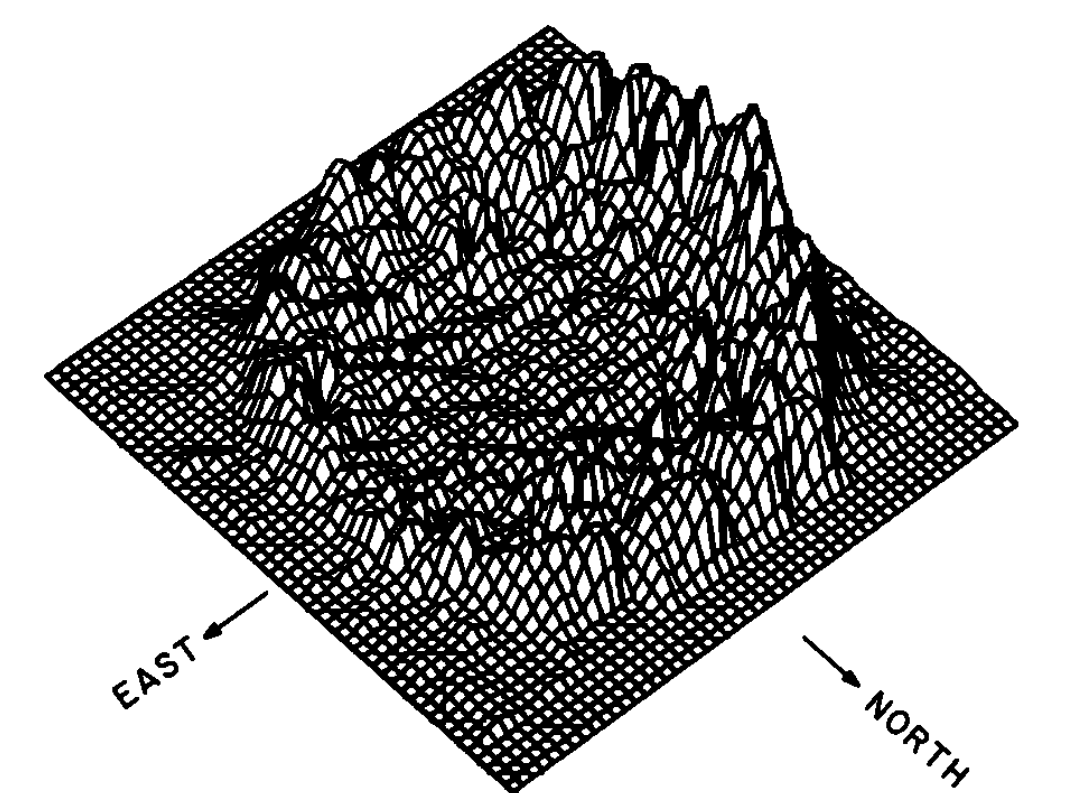
\includegraphics[width=0.48\textwidth]{content/literature_review/figures/sas2_map.png}
            }
        \hfill
         \subfloat[
            EGRET experiment (\cite{Petry05})
         ]{
            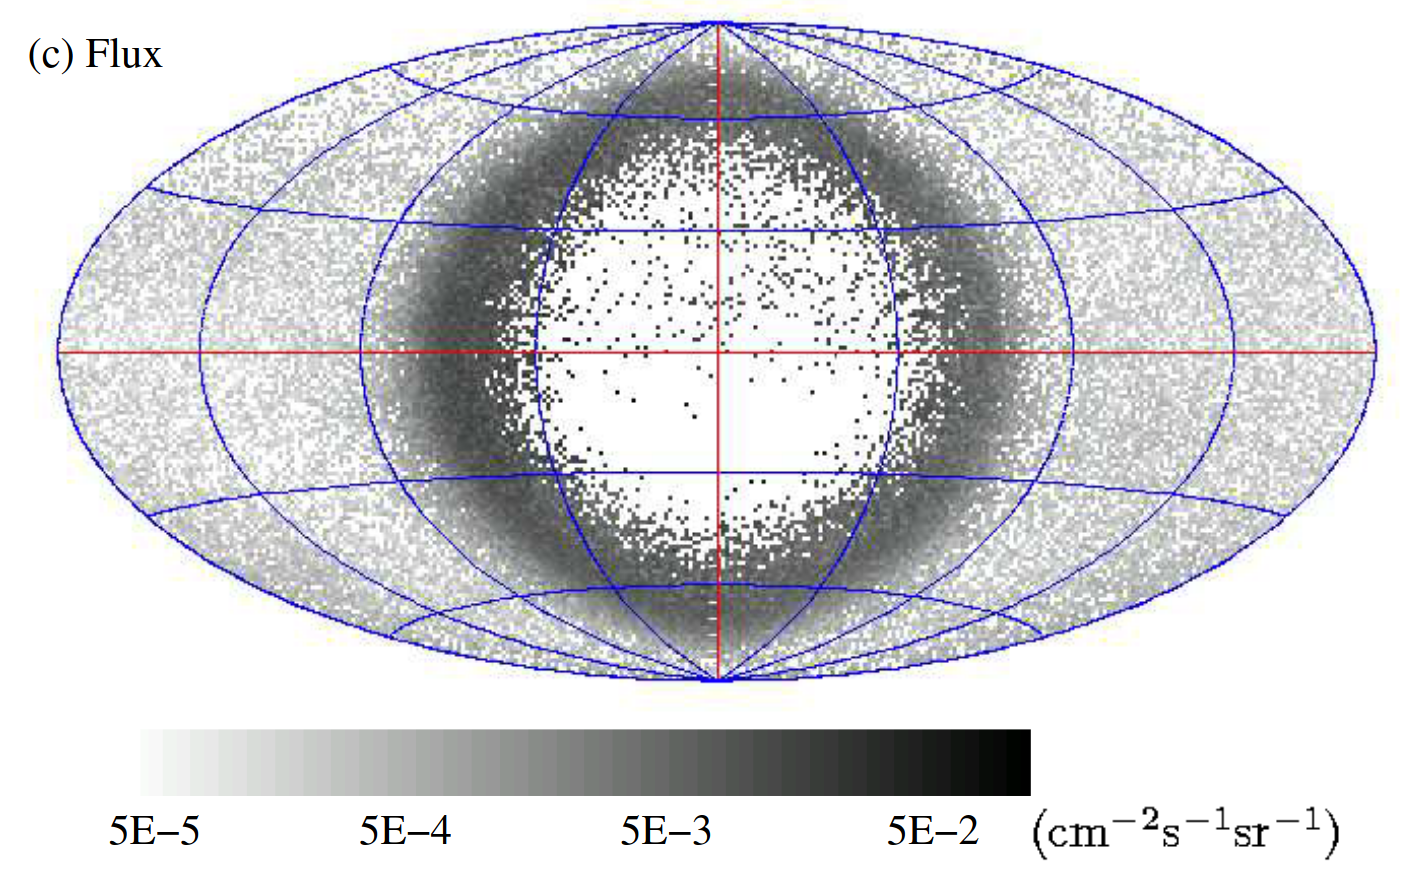
\includegraphics[width=0.48\textwidth]{content/literature_review/figures/egret_map.png}
        }
        \caption{
            The Earth's centered intensity plot from the satellite based observations
        }
       \label{fig:gamma_earth_second_wave}
\end{figure}

% gamma from earth and moon \cite{Morris84}
The previous details are full of so much experimental evidence.
However, \cite{Morris84} put the weights on the assumption of 
bright region as seen as albedo in $\gamma$-ray came from the 
interaction of proton and the atmospheric nuclei. The study
shows the $\gamma$-rays intensity and the variation of air depth 
by differing the zenith angle along limb region as plotted in 
Figure \ref{fig:emit_photon_vs_depth} and \cite{Thompson81} data 
has been exploited in the analysis.

\begin{figure}[h!]
    \centering
    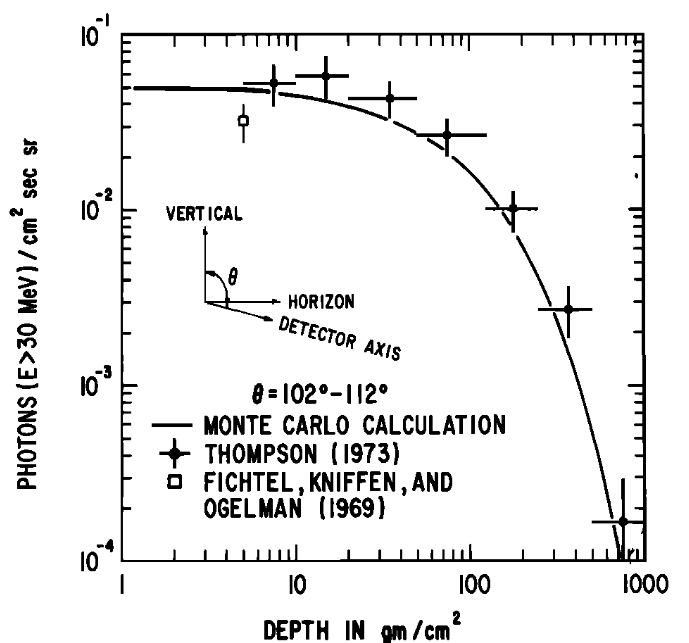
\includegraphics[width=0.6\textwidth]{content/literature_review/figures/morris_photon_vs_depth}
    \caption{
        Calculated $\gamma$-ray intensity with the variation of 
        zenithal angle
        (\cite{Morris84} )
    }
    \label{fig:emit_photon_vs_depth}
\end{figure}

Furthermore, this study computes the $\gamma$-ray spectrum from 
the bright region as seen as albedo from the Earth's limb and 
lunar albedo. The Figure \ref{fig:gamma_spectrum_earth_lunar} 
shows the spectrum from the theoretical calculation. Figure \ref{fig:gamma_spectrum_earth_lunar}a
identify the 2 bounds of the limb's region with an approximated air depth.
Appealingly, another evidence of the solar activity could cause lower arrival CR particles since the propagating magnetic field 
drag a charged particle towards outer space. The distinguishable
spectrum from this phenomenon is demonstrated in
Figure \ref{fig:gamma_spectrum_earth_lunar}b.


\begin{figure}[h!]
    \centering
        \subfloat[
            Earth's limb $\gamma$-ray spectrum
        ]{
            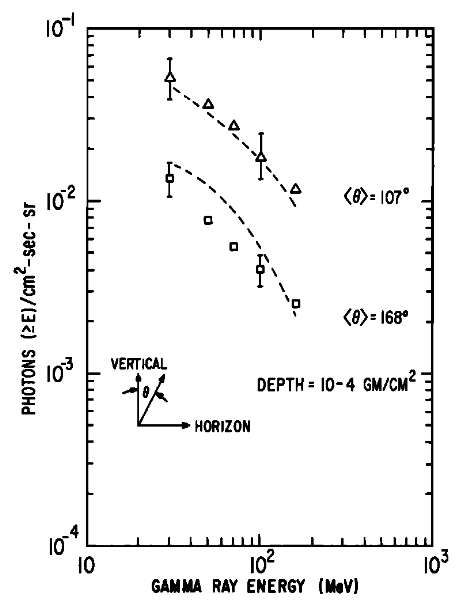
\includegraphics[width=0.48\textwidth]{content/literature_review/figures/morris_earth_spectrum.png}
            }
        \hfill
         \subfloat[
            Lunar's atmospheric $\gamma$-ray spectrum
         ]{
            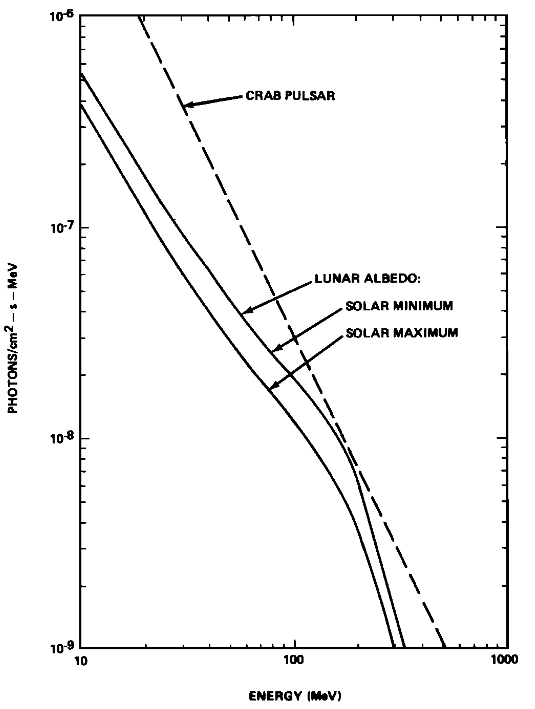
\includegraphics[width=0.48\textwidth]{content/literature_review/figures/morris_lunar_spectrum.png}
        }
        \caption{
            $\gamma$-ray spectrum from proton-nuclei interactions
            (\cite{Morris84})
        }
       \label{fig:gamma_spectrum_earth_lunar}
\end{figure}


%% cr induced gamma-ray Fermi
\begin{figure}[h!]
    \centering
    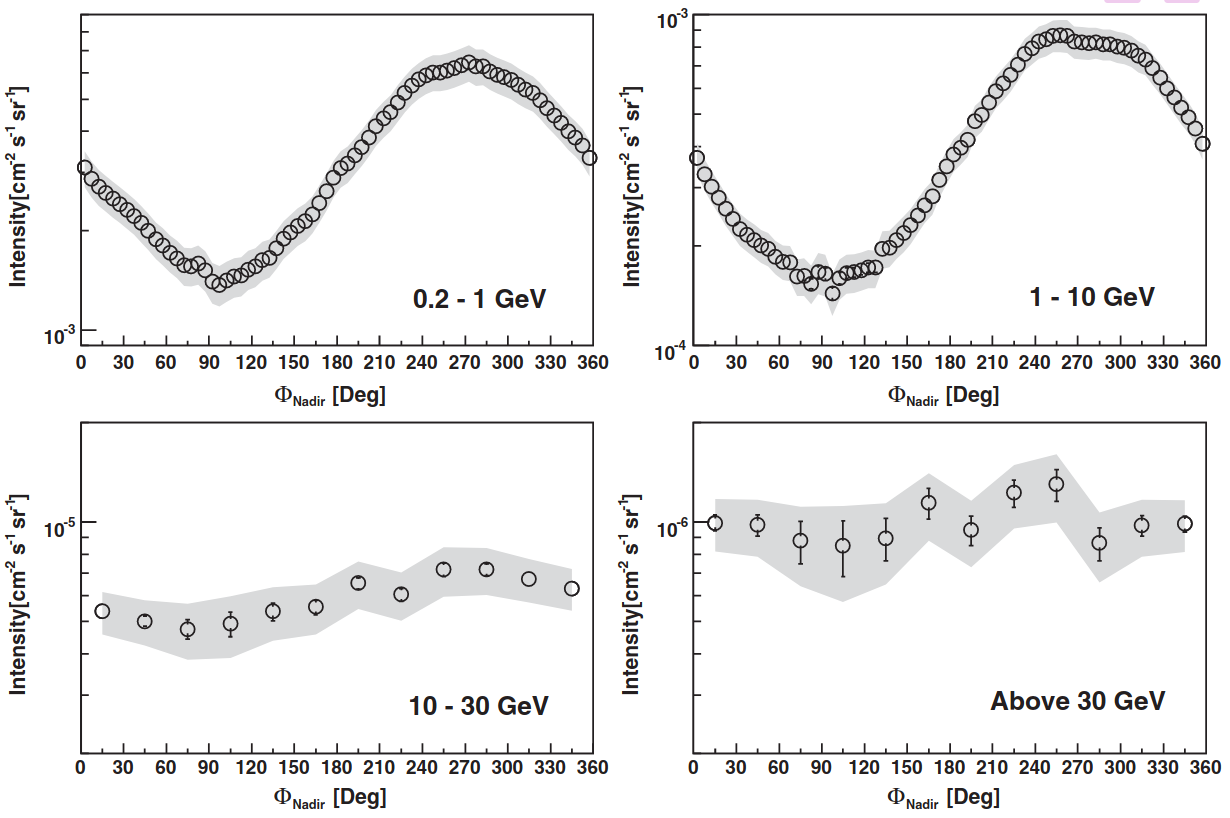
\includegraphics[width=0.9\textwidth]{content/literature_review/figures/fermi_eastwest.png}
    \caption{
        $\gamma$-rays intensity from limb emission in 4 energy ranges
        (\cite{fermilat_gamma_induced})
    }
    \label{fig:fermi_eastwest}
\end{figure}

Not so long after \textit{Fermi}-LAT was launched in the sky. In 2009,
an early examination of the induced $\gamma$-ray emission was 
observed by the most precise $\gamma$-ray detector
\cite{fermilat_gamma_induced}. Since there 
is a huge improvement in the technological side which makes LAT 
capable of detecting high energy $\gamma$-ray from MeV up to TeV.
Another discovery from this study was the East-West effect is highly 
depends on the energy where it was converted from the incident energy of CR particles. The higher energy means the higher rigidity
and it would reflect how hard the magnetic field could bend the trajectory.
The intensity was divided into 4 energy ranges from a few GeV 
to a higher GeV that could be considered as the relativistic scheme 
where the kinetic energy is much higher than the mass as shown 
in Figure \ref{fig:fermi_eastwest}.

% PAMELA proton&He cite:adriani2011pamela
% BESS: p&He cite: bess_experiment
% ams-02 proton cite:AMS02pr2015
% ams-02 helium cite:Heliumflux2015
The objective of this work is to indirectly measure the proton spectrum in 
GeV range. The direct measurement in an early study of high energy 
CR particles such as proton and helium were observed by \cite{bess_experiment}.
Another following experiment is \cite{adriani2011pamela}. Both of 
them still lack the capability to detect such high energy on a scale of 
a hundred GeV. Nevertheless, there is a clue about the breaking energy 
in the proton spectrum with very low statistics and leaves room for further study.


% previous work (indirect measurement) : FermiEarth14
Since there is just a clue from the previous direct observations.
The indirect measurement of CR proton spectrum has been performed in
energy between 90 GeV to 6 TeV by taking advantage of the brightness of
Earth's limb from the collision of incident CR protons (\cite{FermiEarth14}).
The 5 years of $\gamma$-ray data have been exploited by investigating the incident proton spectrum via proton-proton collision model for finding whether CR protons have a breaking point of slope in the power 
law spectrum. The study found that there is a breaking spectral index
in the proton spectrum above 200 GeV 
Nonetheless, Statistical analysis turns out that it is 1$\sigma$
significant level.


Back in 2011, one of the most efficient
space-based CR detectors was launched by the carriage of Endeavor
space shuttle. The detector has been attached to the international space station (ISS). The main mission of AMS-02 is to search an 
antimatter, dark matter from measuring CRs. It can
detect antimatter such as position and antiproton. This detector
is also able to detect other heavyweight nuclei like B, CNO,
Ne, etc. In 2015, a proton spectrum has been directly
reported and found the breaking at 340 GV (\cite{AMS02pr2015})
with very high statistics. Not only the proton but the helium spectrum
is also measured and reported in \cite{Heliumflux2015}. 



% Turning back to the main objective of this work. The core concept 
% is to indirectly measure the proton CR spectrum 
According to the previous study (\cite{FermiEarth14}), 
low statistical significant potentially came from lack of the 
dataset or the methodology from the consequence of indirect
measurement. In this work, a similar study will be performed with 
a larger data size from $\sim$ 9 years of observation. Hopefully, 
the study could answer the first mentioned clue and put the weights
on previous work. Moreover, an improvement of the optimization
process by employing the heuristic optimization as well as the
high performance calculation of the exposure map for a lesser
computational time in $\gamma$-ray spectrum calculation. 